\begin{figure}[t]
\uwsinglespace
\centering
\begin{adjustbox}{max size={.6\textwidth}{.6\textheight}}
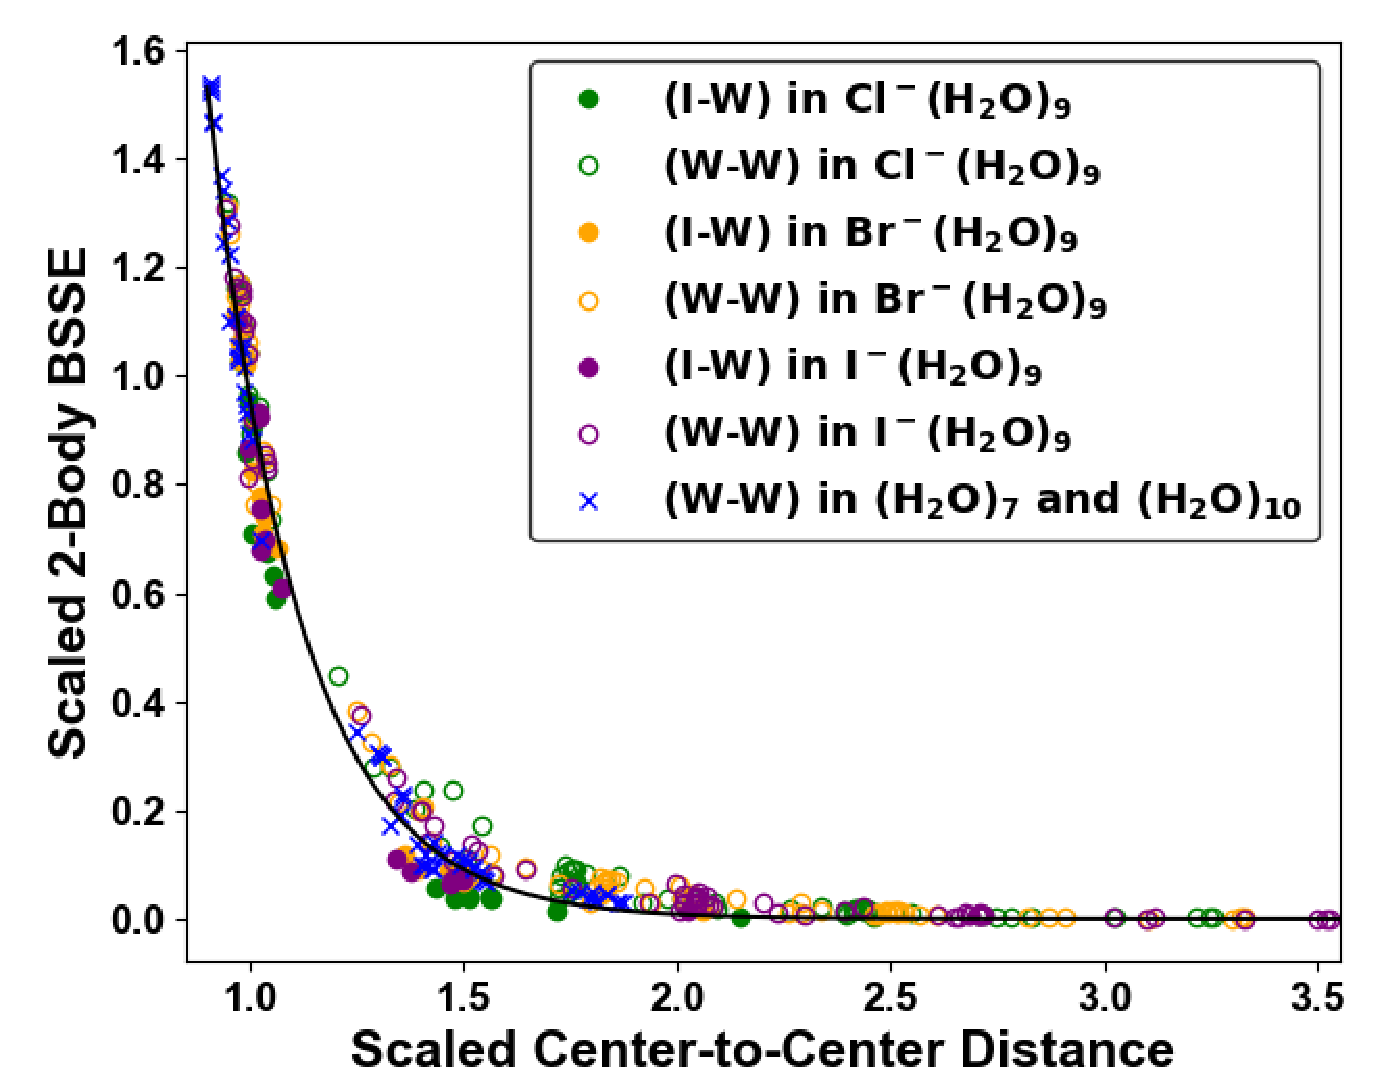
\includegraphics[width=\textwidth]{Figures/Chapter_3/figure_12.pdf}
\end{adjustbox}
\begin{spacing}{1.0}
\caption[Scaled 2-Body BSSE values for all 336 ion-water and water-water dimers cut from \ce{Z^-(H2O)9} where \ce{Z} = \ce{Cl^-}, \ce{Br^-}, and \ce{I^-} as well as two neutral water clusters of \ce{(H2O)7} and \ce{(H2O)_{10}}. Each energy is scaled by the size of the BSSE-correction of the corresponding \ce{Z^-(H2O)} dimer or that of a neutral water dimer. Each distance is scaled by the equilibrium center-to-center distance in those same dimers.]{Scaled 2-Body BSSE values for all 336 ion-water and water-water dimers cut from \ce{Z^-(H2O)9} where \ce{Z} = \ce{Cl^-}, \ce{Br^-}, and \ce{I^-} as well as two neutral water clusters of \ce{(H2O)7} and \ce{(H2O)_{10}}. Each energy is scaled by the size of the BSSE-correction of the corresponding \ce{Z^-(H2O)} dimer or that of a neutral water dimer. Each distance is scaled by the equilibrium center-to-center distance in those same dimers. See text for more detail.}\label{fig:MBE_II_12}
\end{spacing}
\end{figure}